\documentclass{article}

\usepackage{graphicx}% Include figure files

\begin{document}

{\centering \bf \LARGE Proposal for Production of a Lattice QCD Data Visualization Code Base}

\section{Objectives}
These are the objectives for this project
\begin{itemize}
  \item display and manipulate data
  \item learn pyvis and bokeh and python in general.
  \item learn how to co-ordinate and create a code base in a small group.
\end{itemize}

\section{Time-frame}
\begin{itemize}
  \item 1.5 hour sessions a week (usually Friday 10:30 am).
  \item first meeting for planning.
  \item 1 meeting to understand bokeh and pyvis.
  \item 1 meeting to discuss data structure and IO
  \item 3 months to have running version.
  \item review after 3 months to discuss continuation. (first Friday of December)
\end{itemize}



\section{Implementation}

\subsection{Code Structure/Graph}
See fig.~\ref{code_sch}. Data is main class type for reading in data. All our data is inherited from Data.
Our pyvis settings class take in Data object. IO is done in pyvis which links to io in data.
\begin{figure}
  \centering
  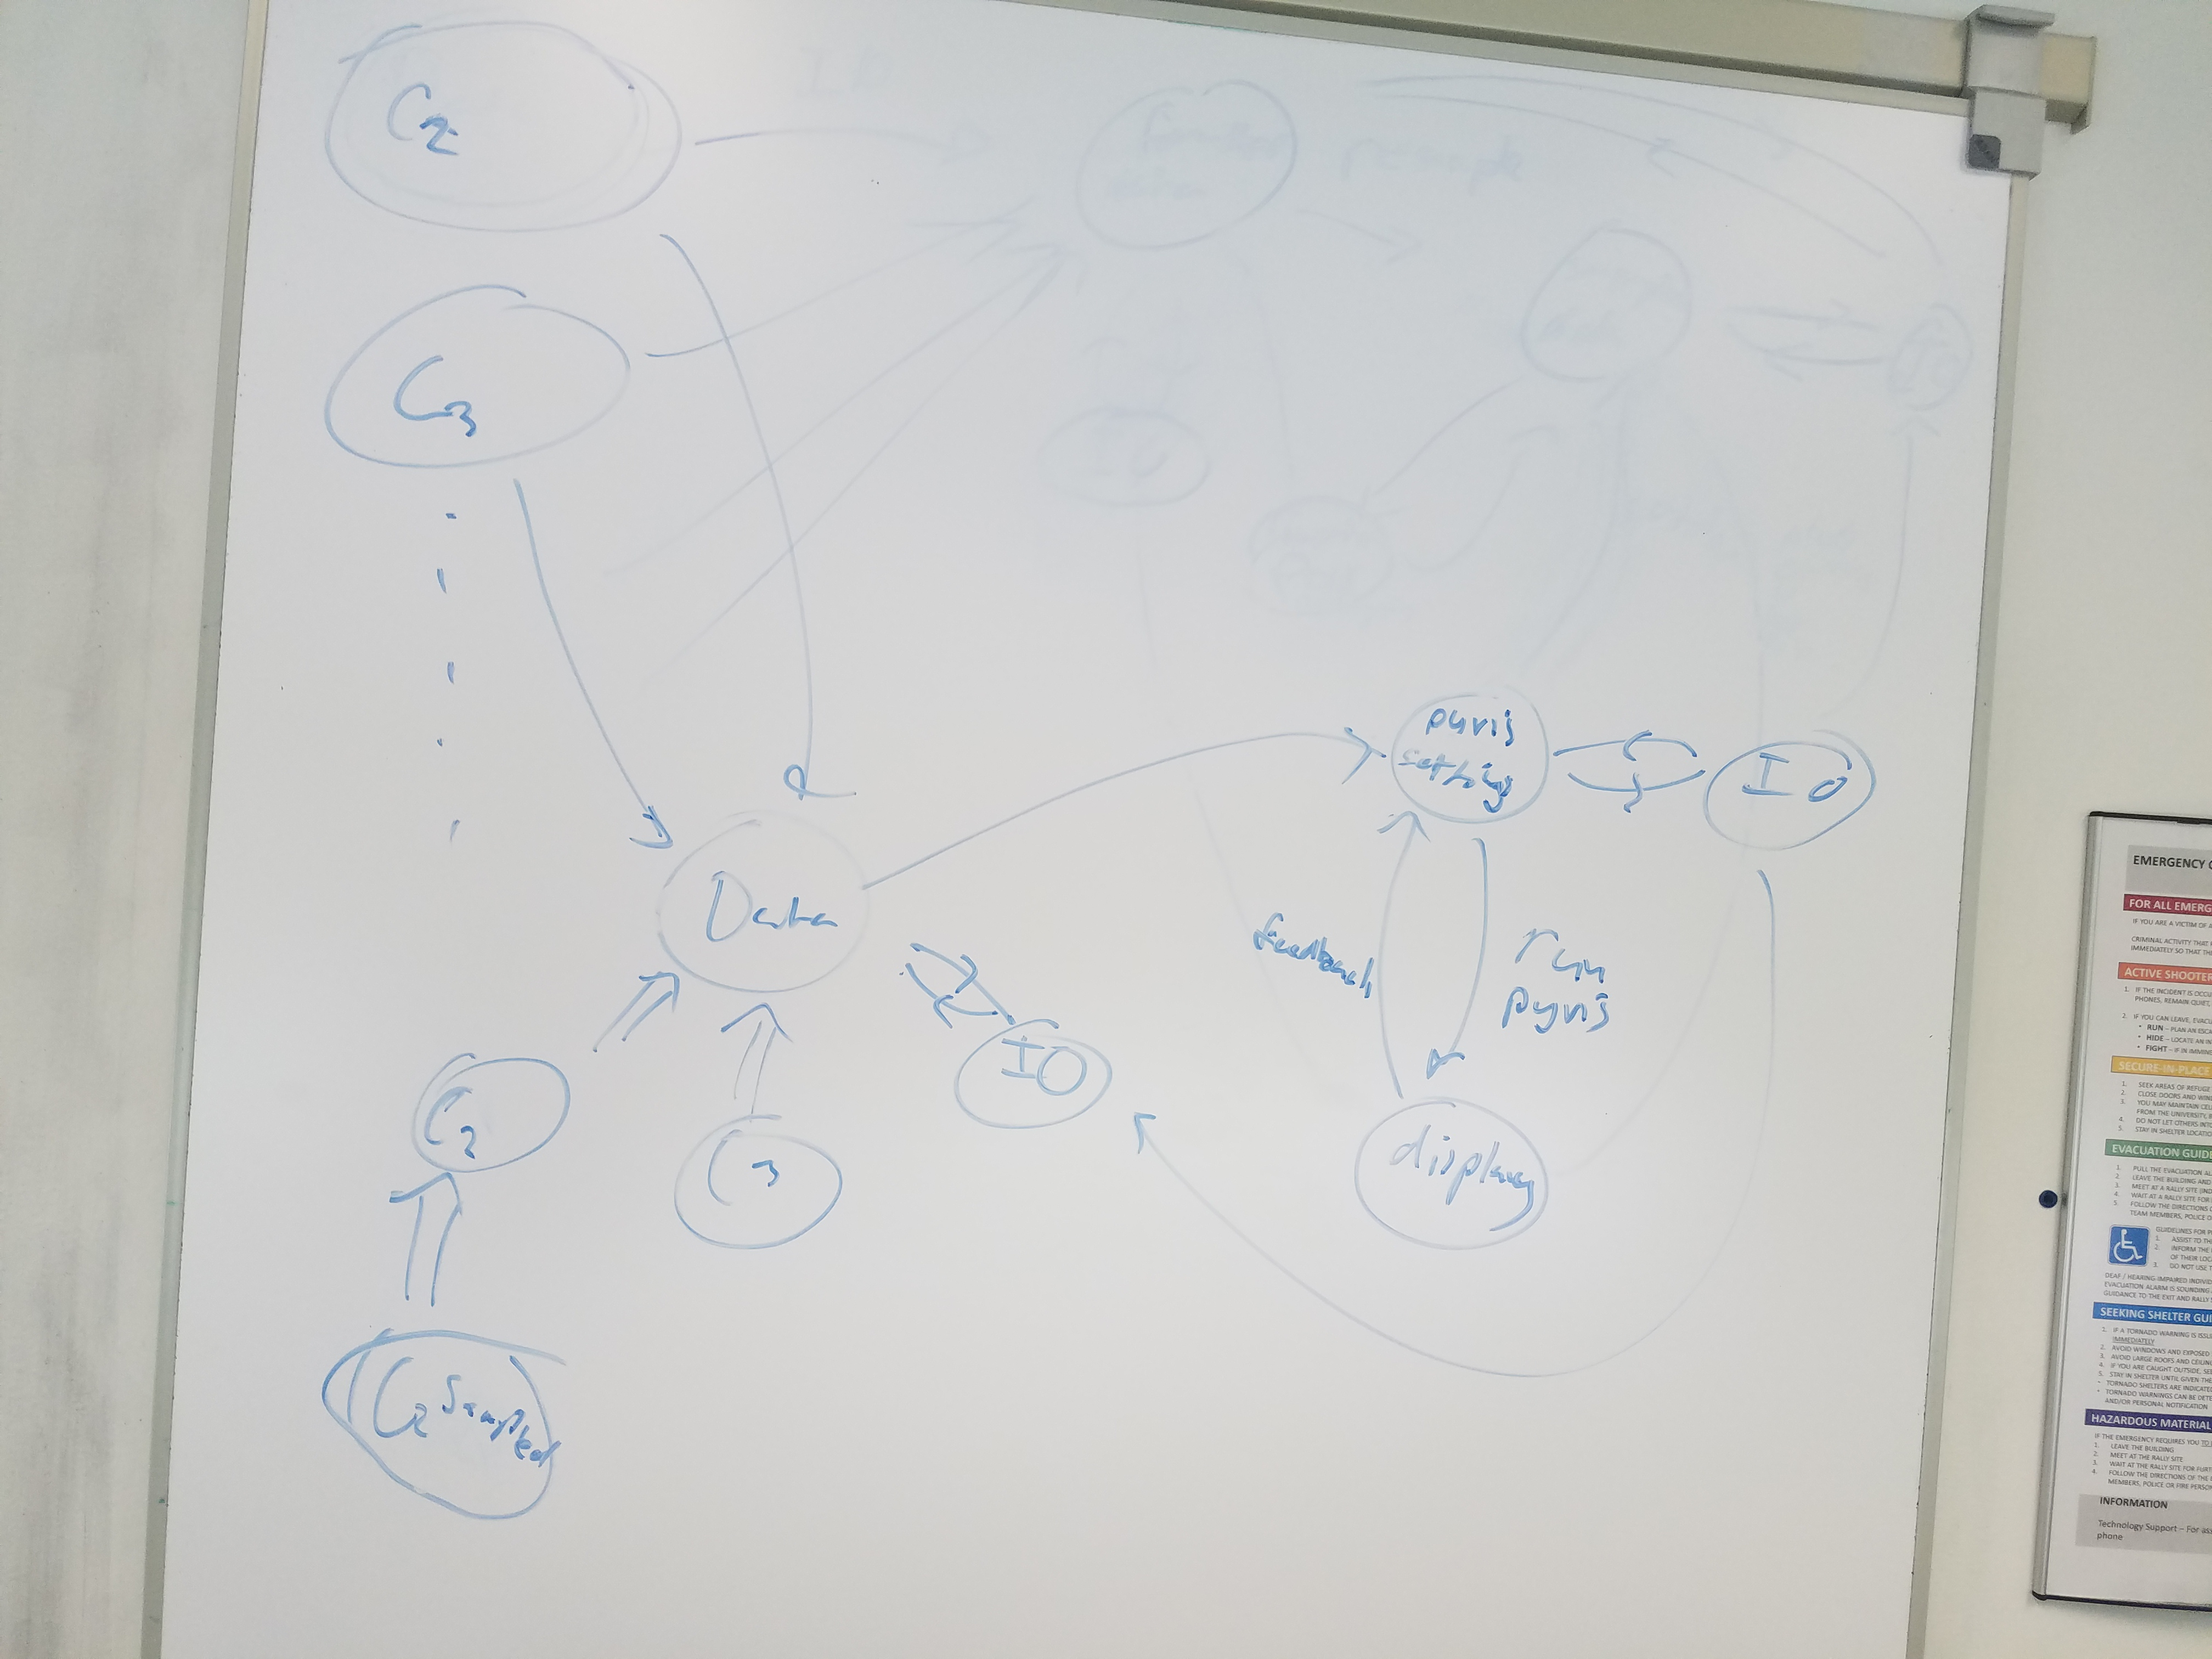
\includegraphics[trim={20cm 0cm 20cm 0cm},clip,width=\linewidth]{/home/jackdra/LQCD/Scripts/group_meeting/Data_Vis_Proj/Plan/Code_Schematic}
  \caption{\label{code_sch}Code schematic for code base. }
\end{figure}
\subsection{Data IO Standardization}
\begin{itemize}
  \item each data type has its own IO functions
  \item hdf5 through pandas
\end{itemize}


\subsection{Packages}
\begin{itemize}
  \item pyvis
  \item bokeh
  \item pandas
  \item numpy
\end{itemize}

\subsection{Debugging, Testing and Test Sets}
\begin{itemize}
  \item Test set of sample data tests the sampled data part of code
  \item test set for raw data to test io and data formatting.
\end{itemize}

\section{Roles/Delegation}
TBA after next two meetings.

\end{document}
